% Recording Bioinformatics Work
%
% A brief set of reasons for why you would want to record your work,
% and record it well.

\subsection{Recording Bioinformatics Work}
\begin{frame}
  \frametitle{Why Do It?}
  \begin{itemize}
    \item Doing bioinformatics is doing science: keep a lab book!
    \item You \emph{will not} remember multiple files, analysis details, etc. in a week/month/six months/a year/three years
    \begin{itemize}
      \item Noble (2009) \url{http://dx.doi.org/10.1371/journal.pcbi.1000424}
      \item Baggerly \& Coombes (2009) \url{http://arxiv.org/pdf/1010.1092.pdf}
    \end{itemize}
  \end{itemize}
  
\includegraphics[width=.6\textwidth]{images/noble_2009_head}
\end{frame}
   
\begin{frame}
  \frametitle{How To Do It? I}
  \begin{itemize}
    \item There is no one correct way, but$\ldots$
    \item Think about data/docs/project structure \textit{before} you start
  \end{itemize}
  \begin{center}
    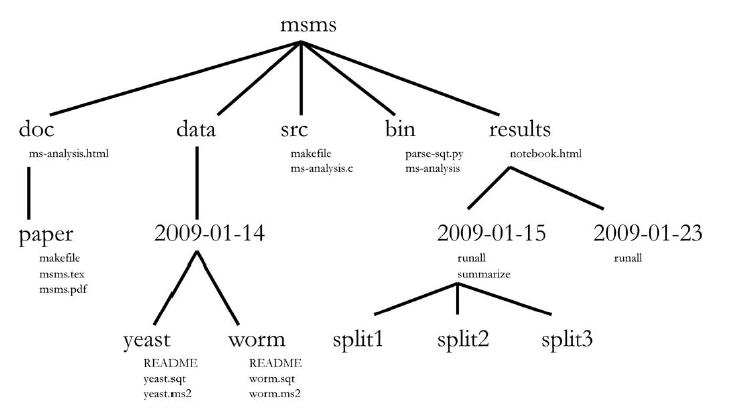
\includegraphics[width=.5\textwidth]{images/project_structure}
    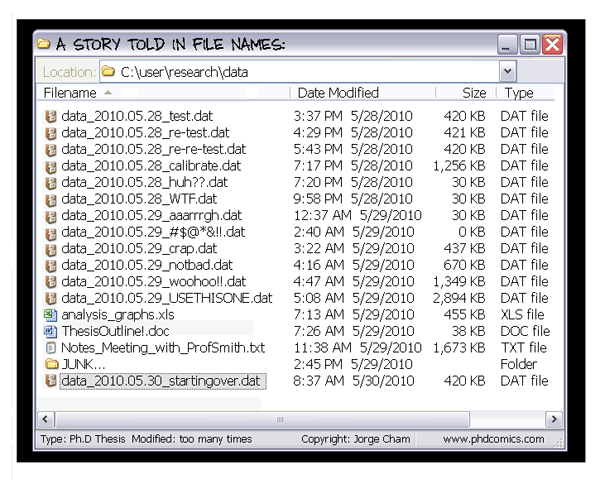
\includegraphics[width=.5\textwidth]{images/phd052810s}
  \end{center}
\end{frame}

\begin{frame}
  \frametitle{How To Do It? II}
  \begin{itemize}
    \item Use plain text where possible
      \item Use version control
      \item Keep backups
      \item Different tools suit different purposes: code \textit{vs.} data \textit{vs.} analysis \textit{vs.} $\ldots$
      \item Find a way that works \emph{for you}.
  \end{itemize}
\end{frame}

\begin{frame}
  \frametitle{How To Do It? III}
  \begin{itemize}
    \item Reproducibility is key!
    \item Scripts and pipelines are better for this than notes of what you did
    \begin{itemize}
      \item Also better for version control, and reuse
    \end{itemize}
    \item Avoid unnecessary duplication
    \begin{itemize}
      \item Someone else may have solved your problem
      \item One (backed up) read-only copy of raw data, keep analyses separate
    \end{itemize}
  \end{itemize}
\end{frame}
